\chapter{Introduction}
\section{Problem statement}
Sports and games have been around the world forever. People used to decide, and still do, about their qualities based on all kinds of tournaments. 

Beating all other teams and winning tournaments seemed to be satisfying enough to decide what team is the best up until the year of 1959, when Arpad Elo came up with his statistical-based ranking algorithm for rating chess players \citep{Eloratingchessplayerspresent1978}. Except chess games, the algorithm has found its applications in different sports as well as in completely different fields.

Even though the Elo rating system has shown to be suitable for chess games, it had not necessarily found its way to other sports. People have come up with various ranking systems or variations of Elo in order to adapt to different sports. With the growth of massively multiplayer online computer gaming, much more sophisticated systems have been created to maximize the player's enjoyment gained from playing a game.

Rating systems introduce the possibility of building a ladder of players, reflecting their results and leading to increased competitiveness. Moreover, rating systems allow the game to match similarly strong players, leading to more balanced and therefore more enjoyable matches. Finally, the system's ability to predict future games can lead to interesting analyses. Overall, good rating systems improve the overall quality of a game leading to a better gaming experience, which obviously makes such game more desired.

Furthermore, rating systems are not limited to be used only in sports and gaming. As \citet{RainieUseOnlineRating2004} shows, plentiful of useful applications have been implemented, such as Google's famous PageRank algorithm \citep{PagePageRankcitationranking1998} used to rank quality of web pages, Amazon's products and sellers ratings \citep{ZhangMiningmillionsreviews2012} to detect the relevance of a product and reliability of a seller, or movie recommendation system used at Neflix \citep{FernandezRecommendationSystemNetflix2018}.

This thesis focuses on applications of several rating systems in soccer with the objective of improving their ability to predict future matches based on players' ratings. In order to achieve that, the results of numerous ranking algorithms are evaluated and then possible methods that lead to the improvement of the prediction ability are introduced. Finally, in \autoref{ch:realisation}, a description of the demo for ranking players and teams is provided, alongside with description of the API.

\section{Data analysis}
\label{sec:data_analysis}
Ranking algorithms are applied on soccer data taken from Kaggle's European Soccer Database, which provides the following \citep{EuropeanSoccerDatabase} data.
\begin{itemize}
\item Over 25 000 matches
\item Over 10 000 players
\item 11 European countries
\item Seasons from 2008 to 2016
\item Players' and teams' attributes
\item Team line up
\item Betting odds by bookkeepers
\item Detailed match events
\end{itemize}

Since not every match in the dataset is provided with all eleven players on each team, matches have to be checked for the suitability during preprocessing of the data, which leads to a final number of 21374 useful matches with following distribution of wins, loses and draws from the perspective of home team.

\begin{figure}[H]
\centering
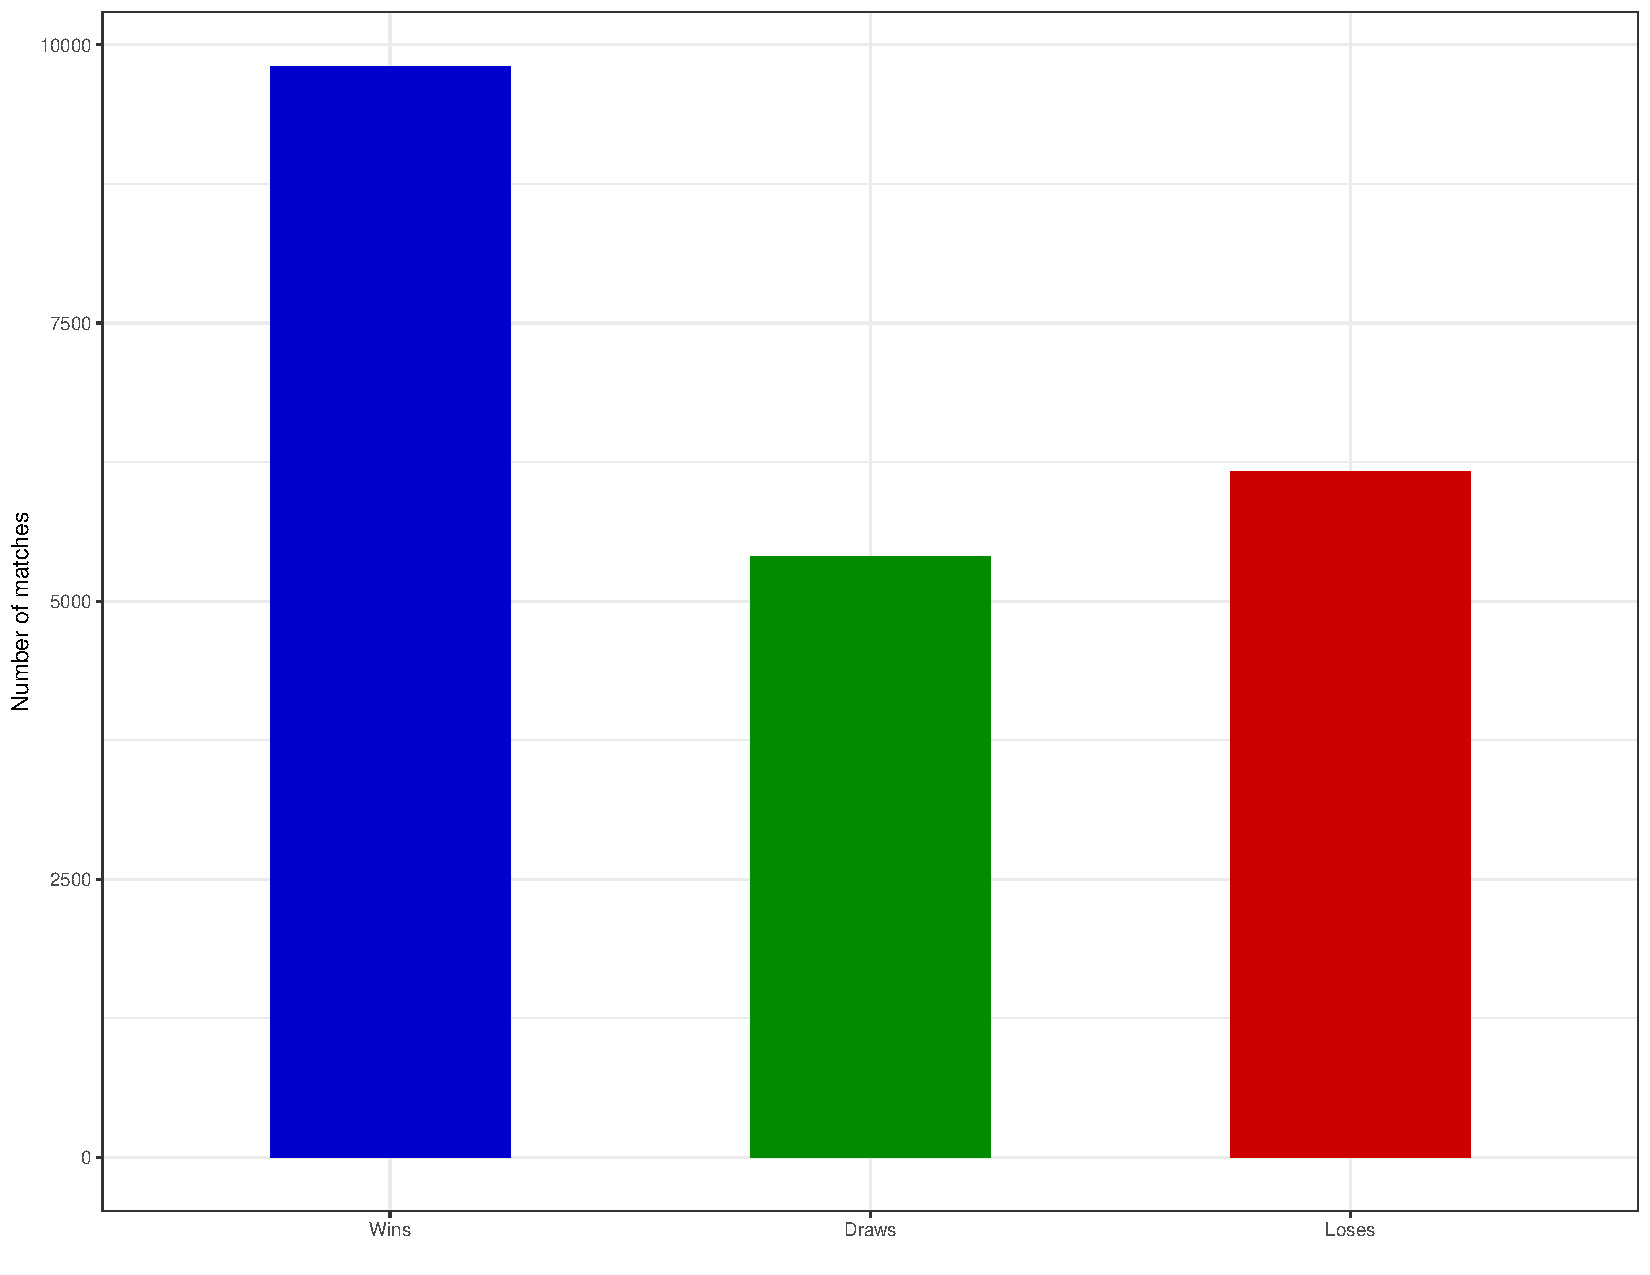
\includegraphics[width=.8\linewidth]{figs/match_distribution}
\caption{Distribution of outcomes}
\label{fig:match_distribution}
\end{figure}

It can be observed from the \autoref{fig:match_distribution} that teams playing on their home ground tend to win more matches. This is called the \textbf{home-team advantage} and is more thoroughly analyzed by \citet{BialkowskiWinHomeDraw}. To underpin the home-team advantage phenomena, distribution of scored goals throughout the matches follows.

\begin{figure}[H]
\begin{minipage}[b]{0.49\textwidth}
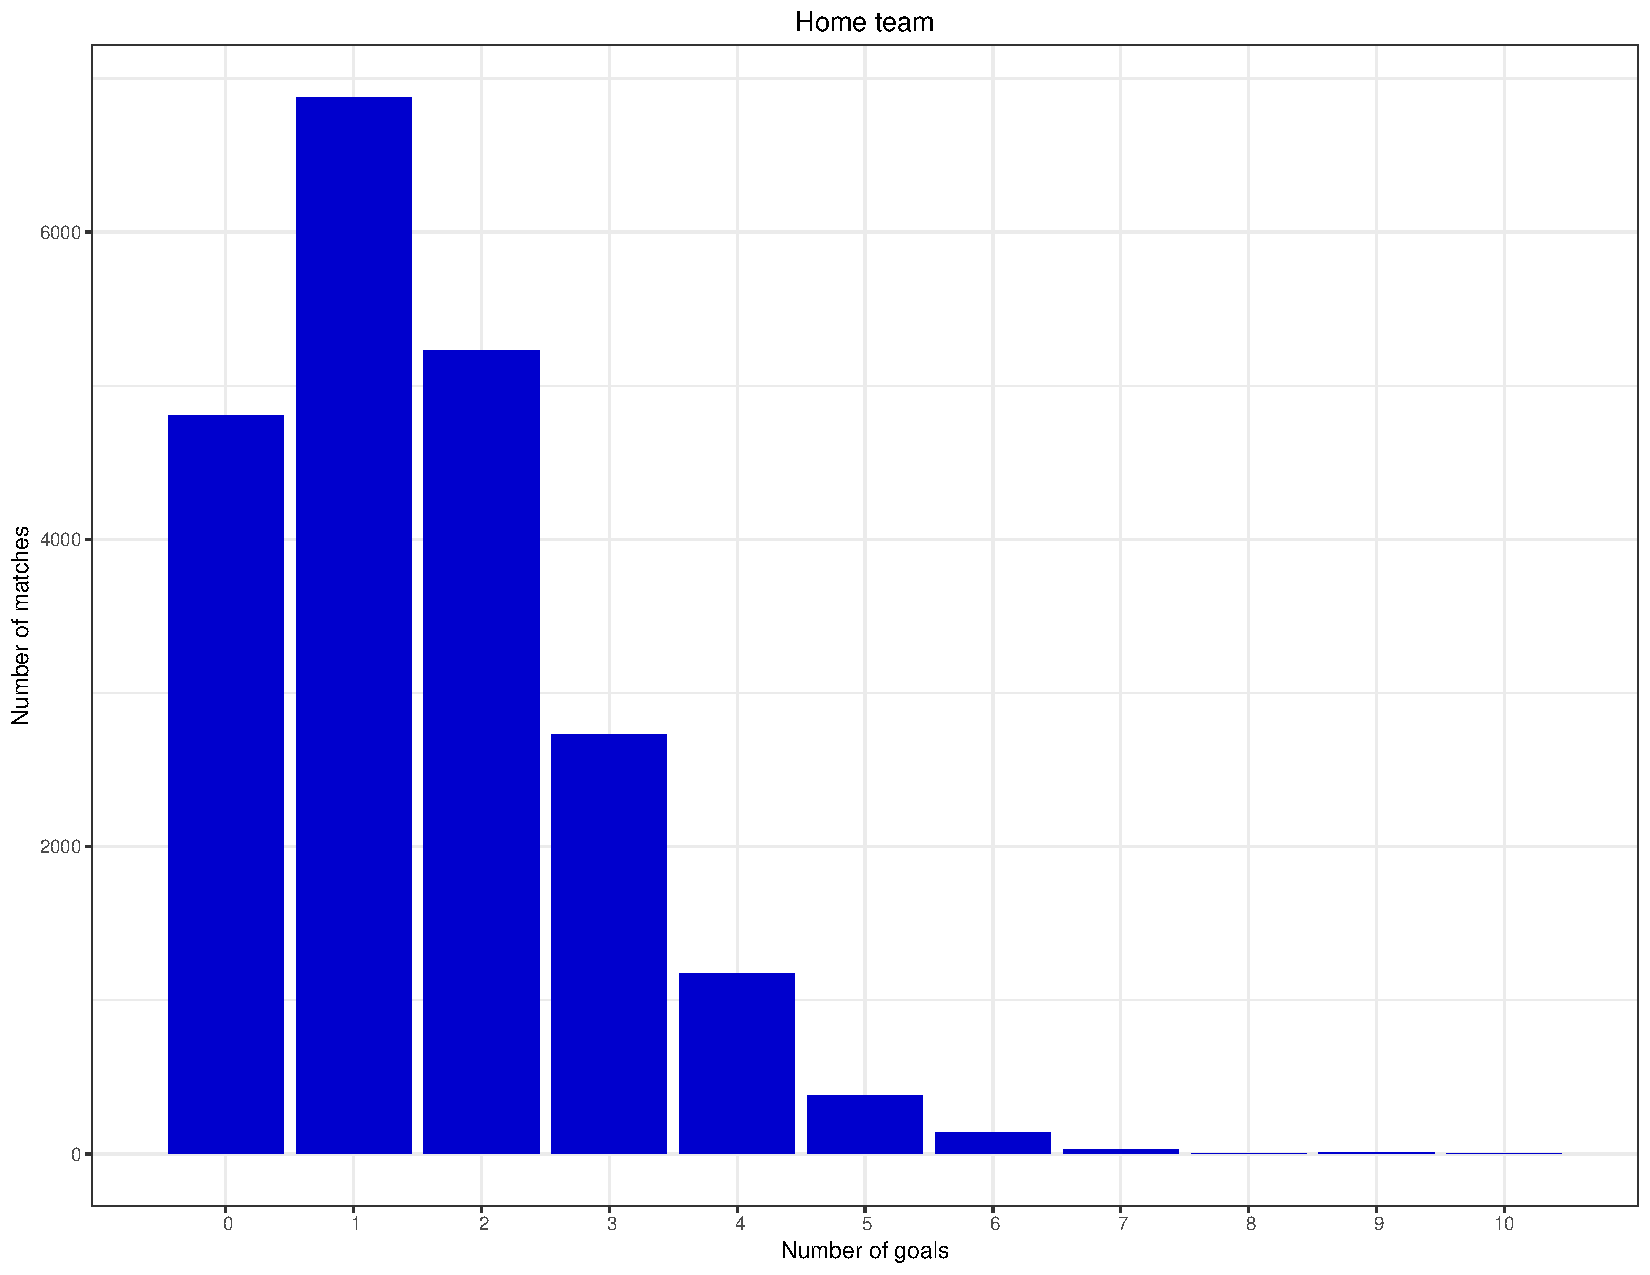
\includegraphics[width=\textwidth]{figs/goal_distribution_home}
\end{minipage}
\hfill
\begin{minipage}[b]{0.49\textwidth}
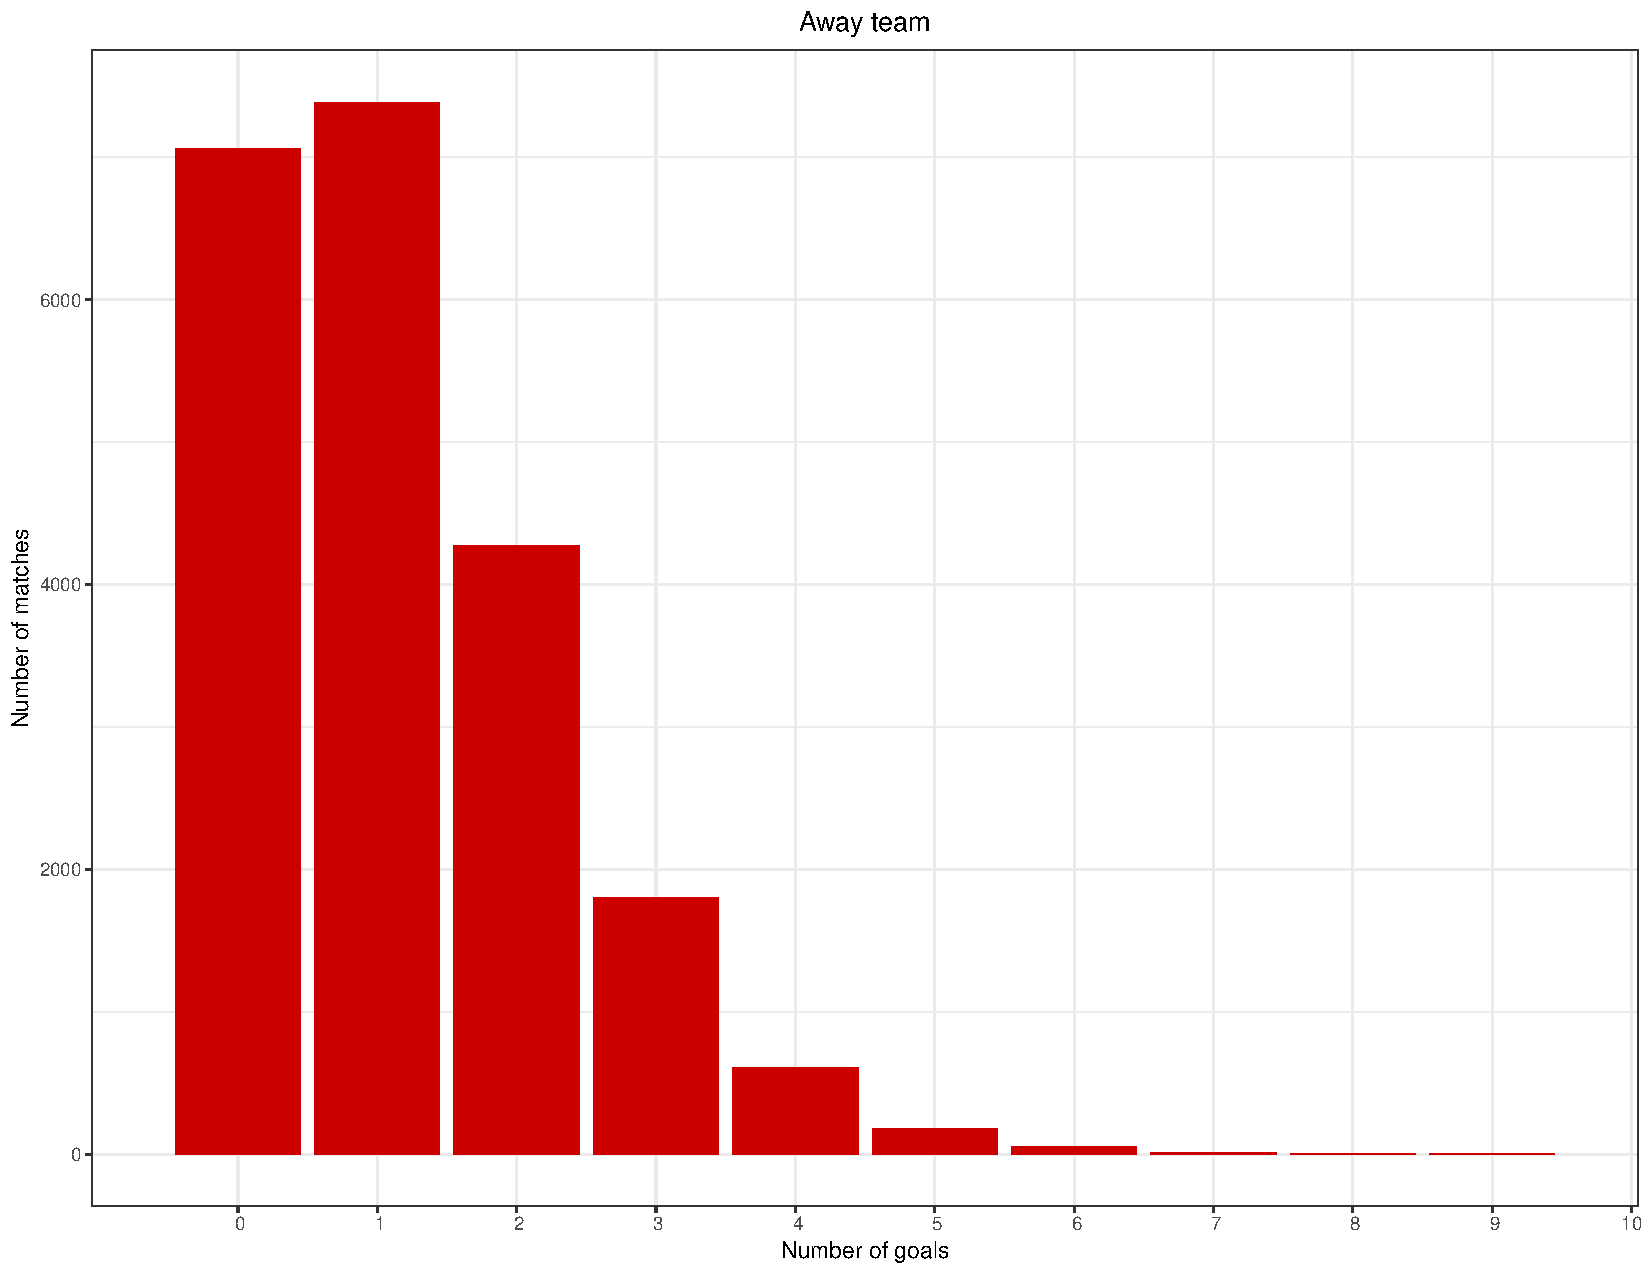
\includegraphics[width=\textwidth]{figs/goal_distribution_away}
\end{minipage}

\vspace{0.5cm}

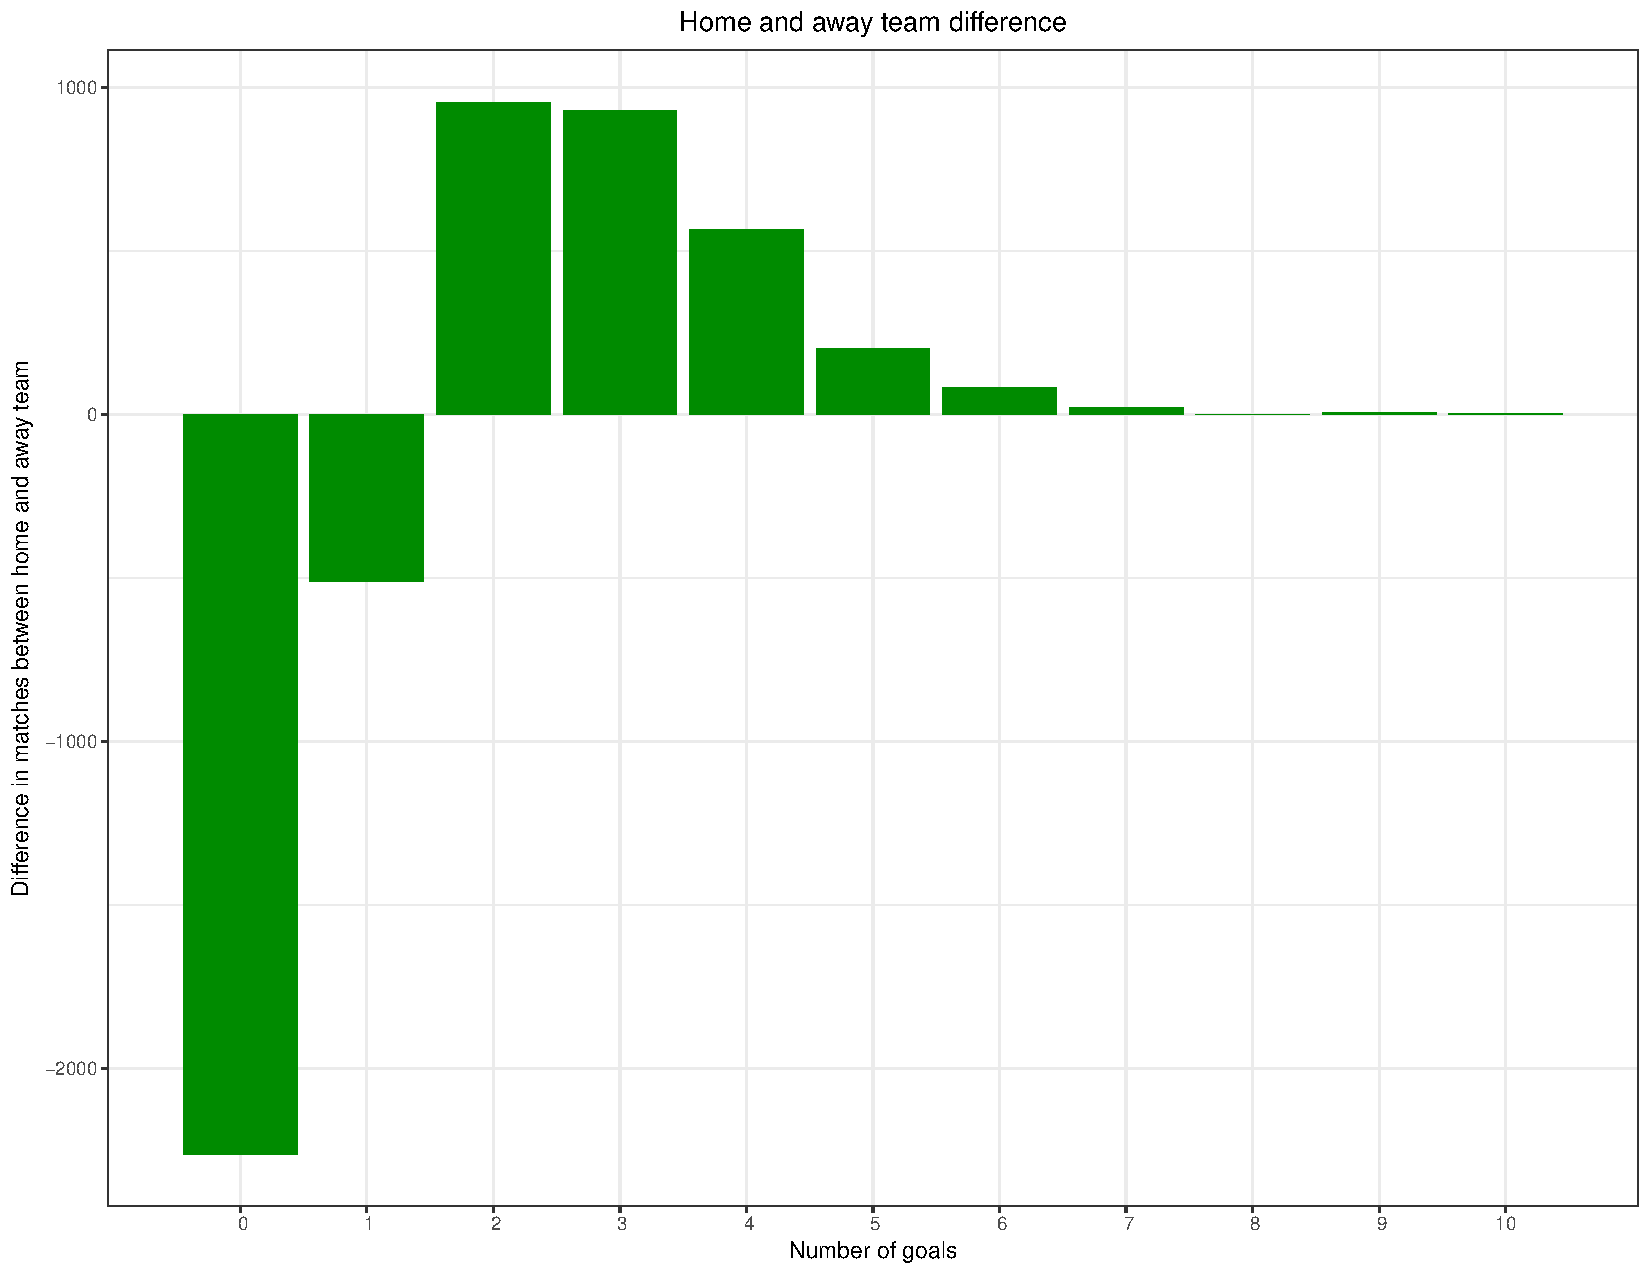
\includegraphics[width=.49\textwidth]{figs/goal_distribution}
\caption{Distribution of scored goals}
\end{figure}

Furthermore, while the away team scores only about $1.18$ goals on an average game, the home team manages to score $1.56$ goals.

Among the players' attributes provided by the dataset, there is the overall rating attribute, providing a rough estimation of player's overall skill based on his recent performance on a $[0, 100]$ scale. Such estimate can be normalized onto a more suitable interval to provide given algorithm with initial players' ratings, possibly leading to faster detection of their true skill.

\begin{figure}[H]
\centering
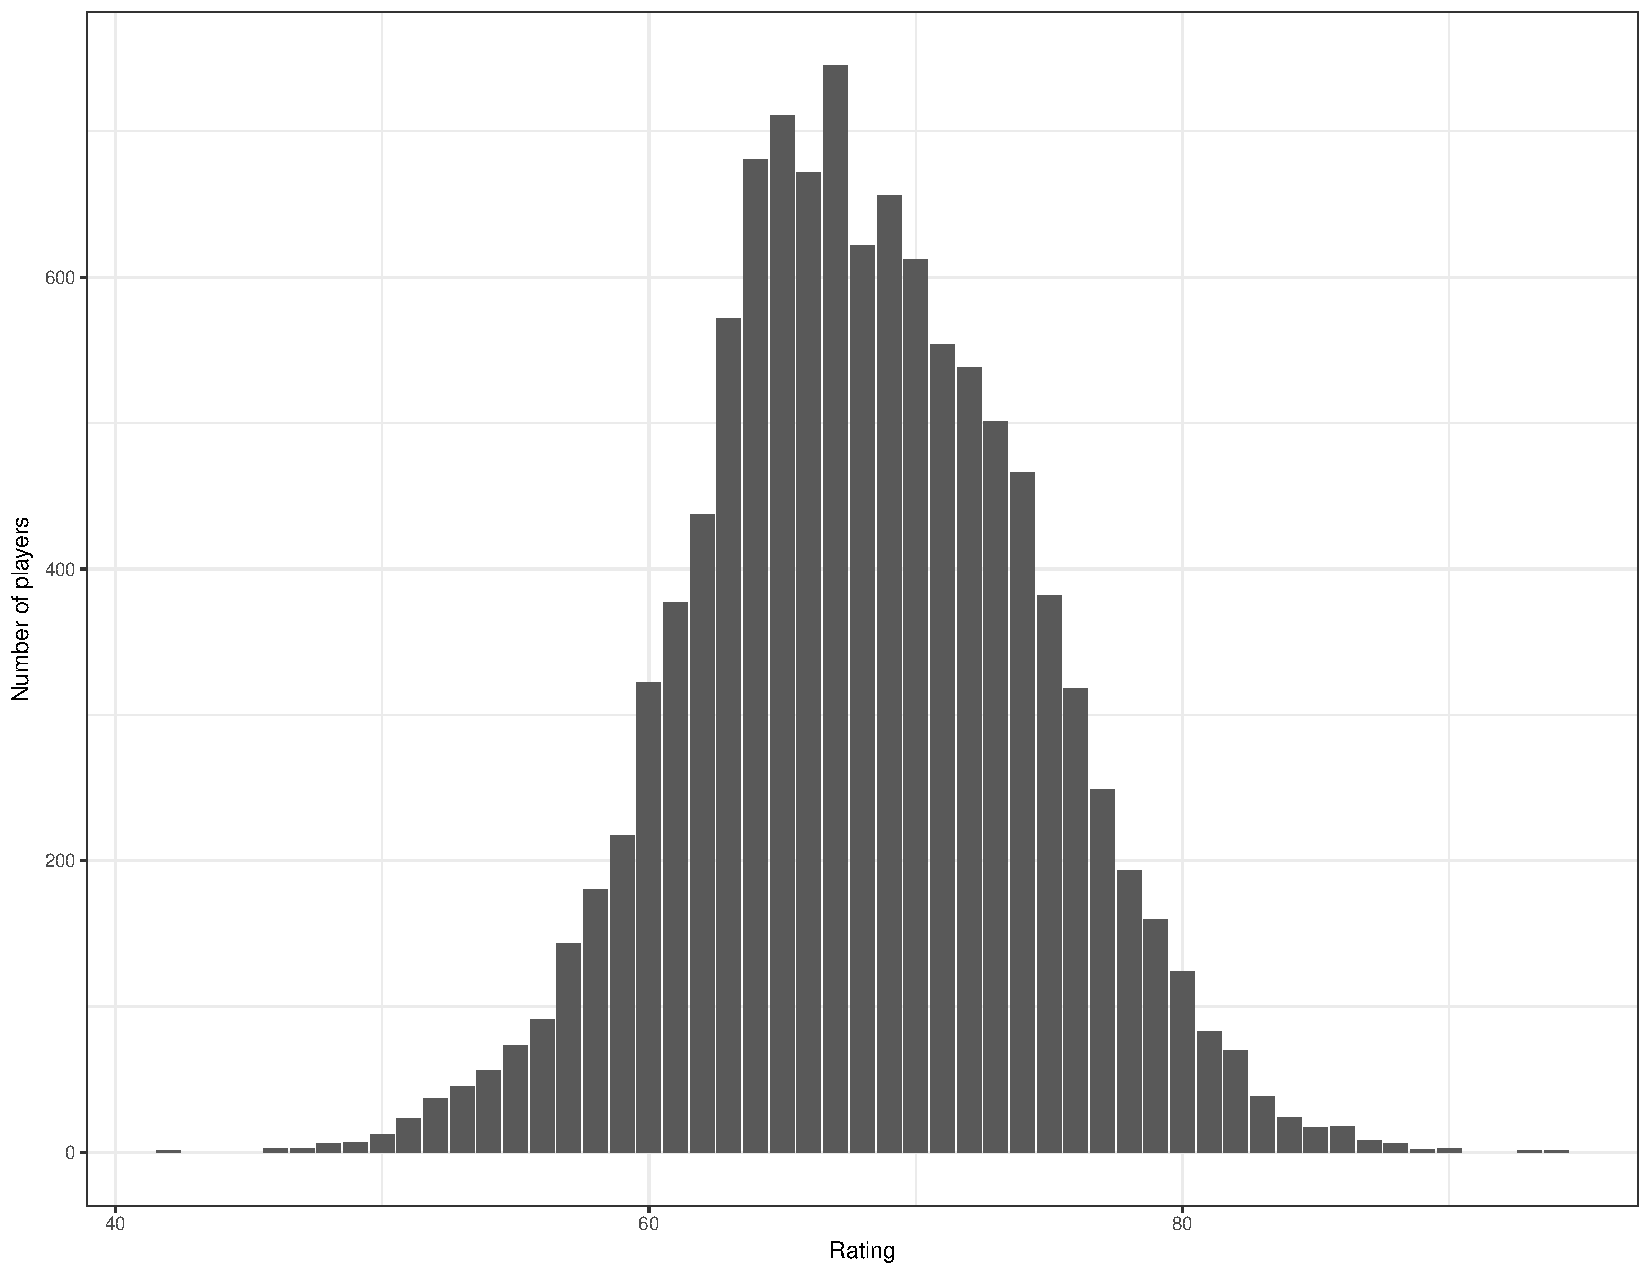
\includegraphics[width=.8\linewidth]{figs/overall_rating_distribution}
\caption{Distribution of overall rating attribute}
\end{figure}

An interesting follow-up statistic is the distribution of goals in given outcome for both home and away teams. \autoref{table:goals_per_outcome} shows such statistic recalculated to number of goals per game.

\begin{table}[H]
\caption{Table of goals per game with respect to outcome}
\label{table:goals_per_outcome}
\centering
\begin{tabular}{| r | c | c | c |}
\hline
& Win & Draw & Lose \\ \hline
Home team & 2.461 & 1.003 & 0.605 \\ \hline
Away team & 2.319 & 1.003 &  0.551 \\ \hline
\end{tabular}
\end{table}

Follows a graphical representation of the same statistic.

\begin{figure}[H]
\caption{Graphical representation of goals per game with respect to outcome}
\centering
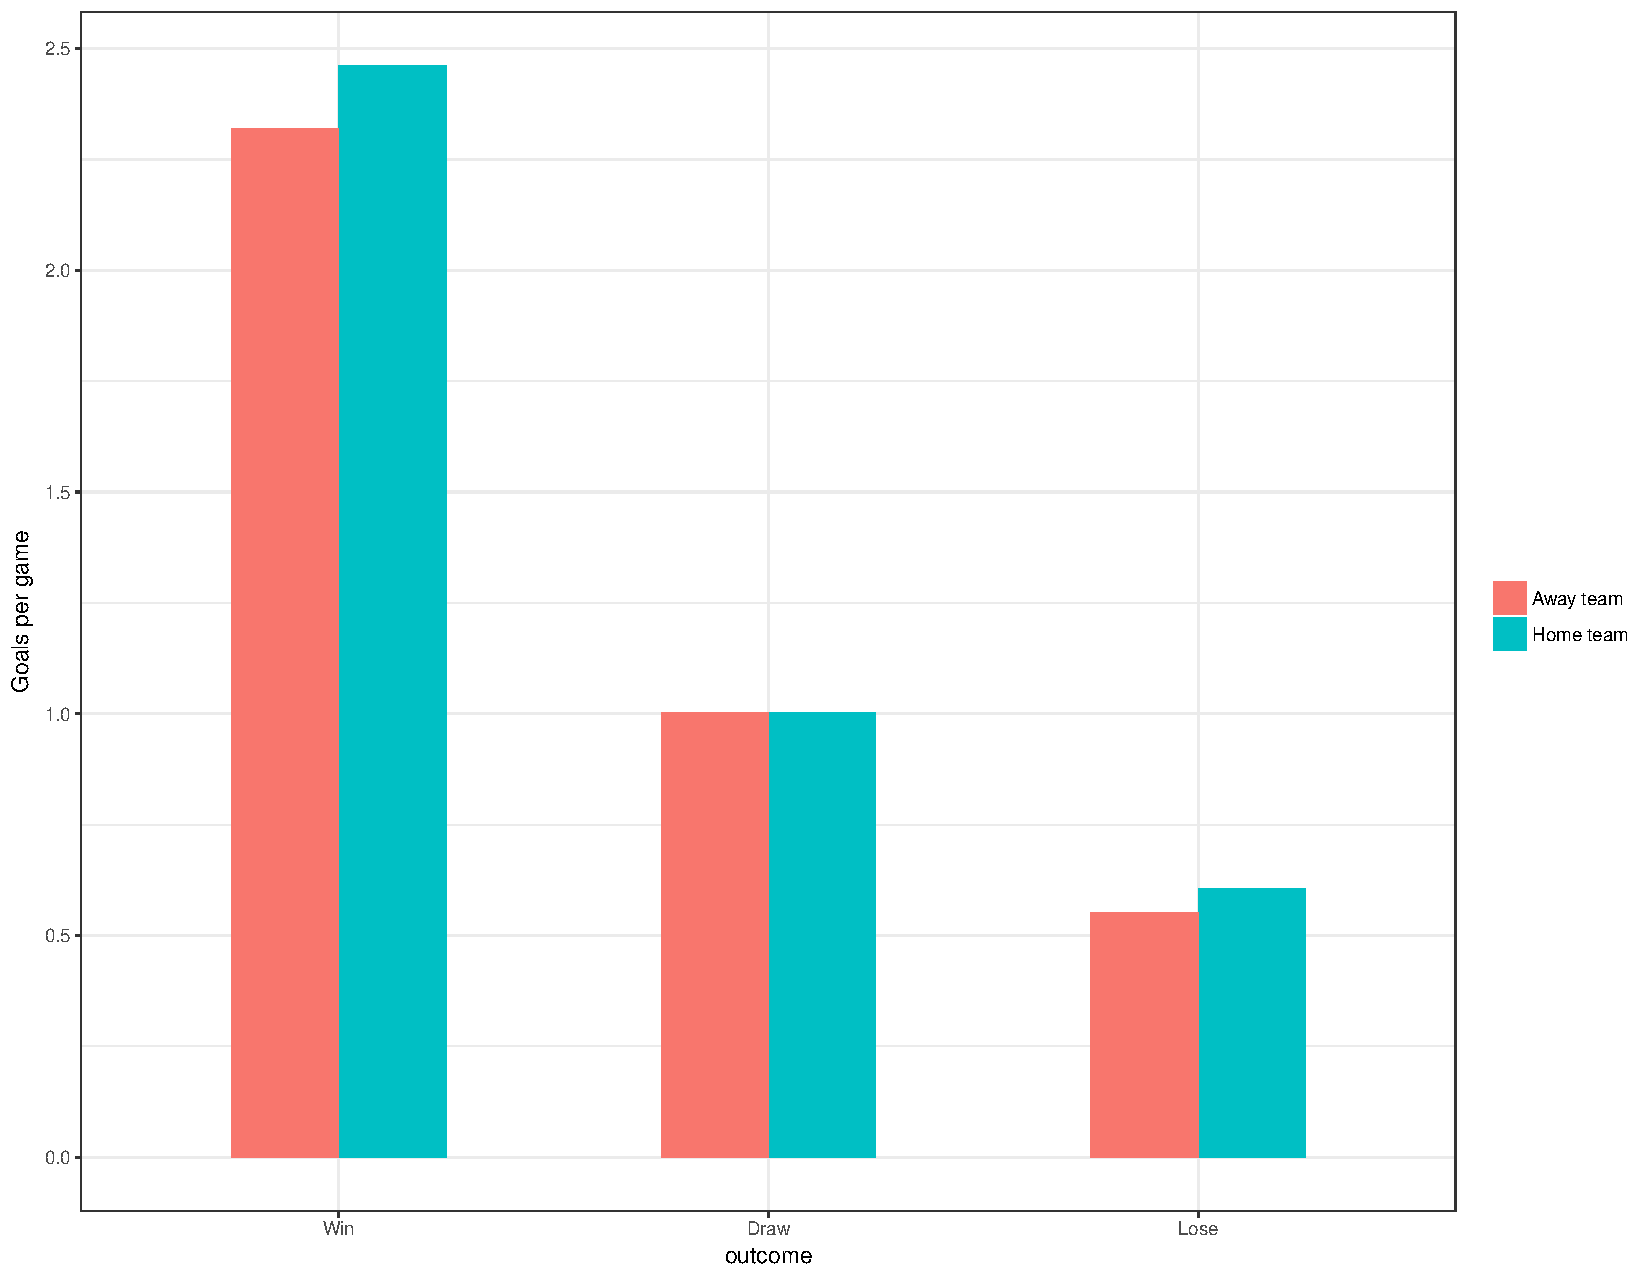
\includegraphics[width=0.8\textwidth]{figs/goals_per_game}
\end{figure}

\section{Measuring skill}
Before the description of specific rating systems, a brief introduction to skill measuring is relevant.

Skill is a relative measure that expresses how well does a player perform in given sport. When comparing two players, it is reasonable to say that the player with highest skill is more probable to defeat the other player. Therefore, skill can be perceived as a relative probability of winning, as introduced by \citet{BradleyRankAnalysisIncomplete1952}.

\begin{equation*}
P(i > j) = \frac{p_i}{p_i + p_j}.
\label{eq:bradley_terry}
\end{equation*}

The model expresses the preference of individual $i$ to individual $j$, with their skills represented as $p_i > 0$ and $p_j > 0$, respectively. A derivation of the Bradley-Terry model will be provided in \ref{sec:multilayer_perceptron}.

Measuring one's skill in games like chess is a lot more complicated than in other sports, where results can be interpreted using an absolute value. For instance, in 100 meter dash, the runner's skill is measured by the time he made. It does not matter who was he competing against, the time is an absolute measure to measure his skill by. However, in sports like chess, players compete against each other and the outcome strictly depends on the skill of player's opponent, which makes measurement methods such as number of victories totally unsuitable.

In order to measure skill of chess players, \textbf{rating} has been introduced. Rating is not measured in any units and therefore only provides information when compared to another player's rating. As capturing a player's skill by a single number may seem peculiar, note that perceiving rating as a random variable is much more appropriate. The number itself then represents the mean of the random variable's distribution, and therefore it is most probable that the player's true skill equals to his rating. The actual distribution of such random variable depends on the standard deviation, which can be variable according to the certainty of the system about the rating.

\examplespace
\begin{example}
Perceiving player's skill as a random variable of the standard normal distribution, skills of players A and B of ratings -0.4 and 0.7, respectively, could be visualized as follows.

\begin{figure}[H]
\centering
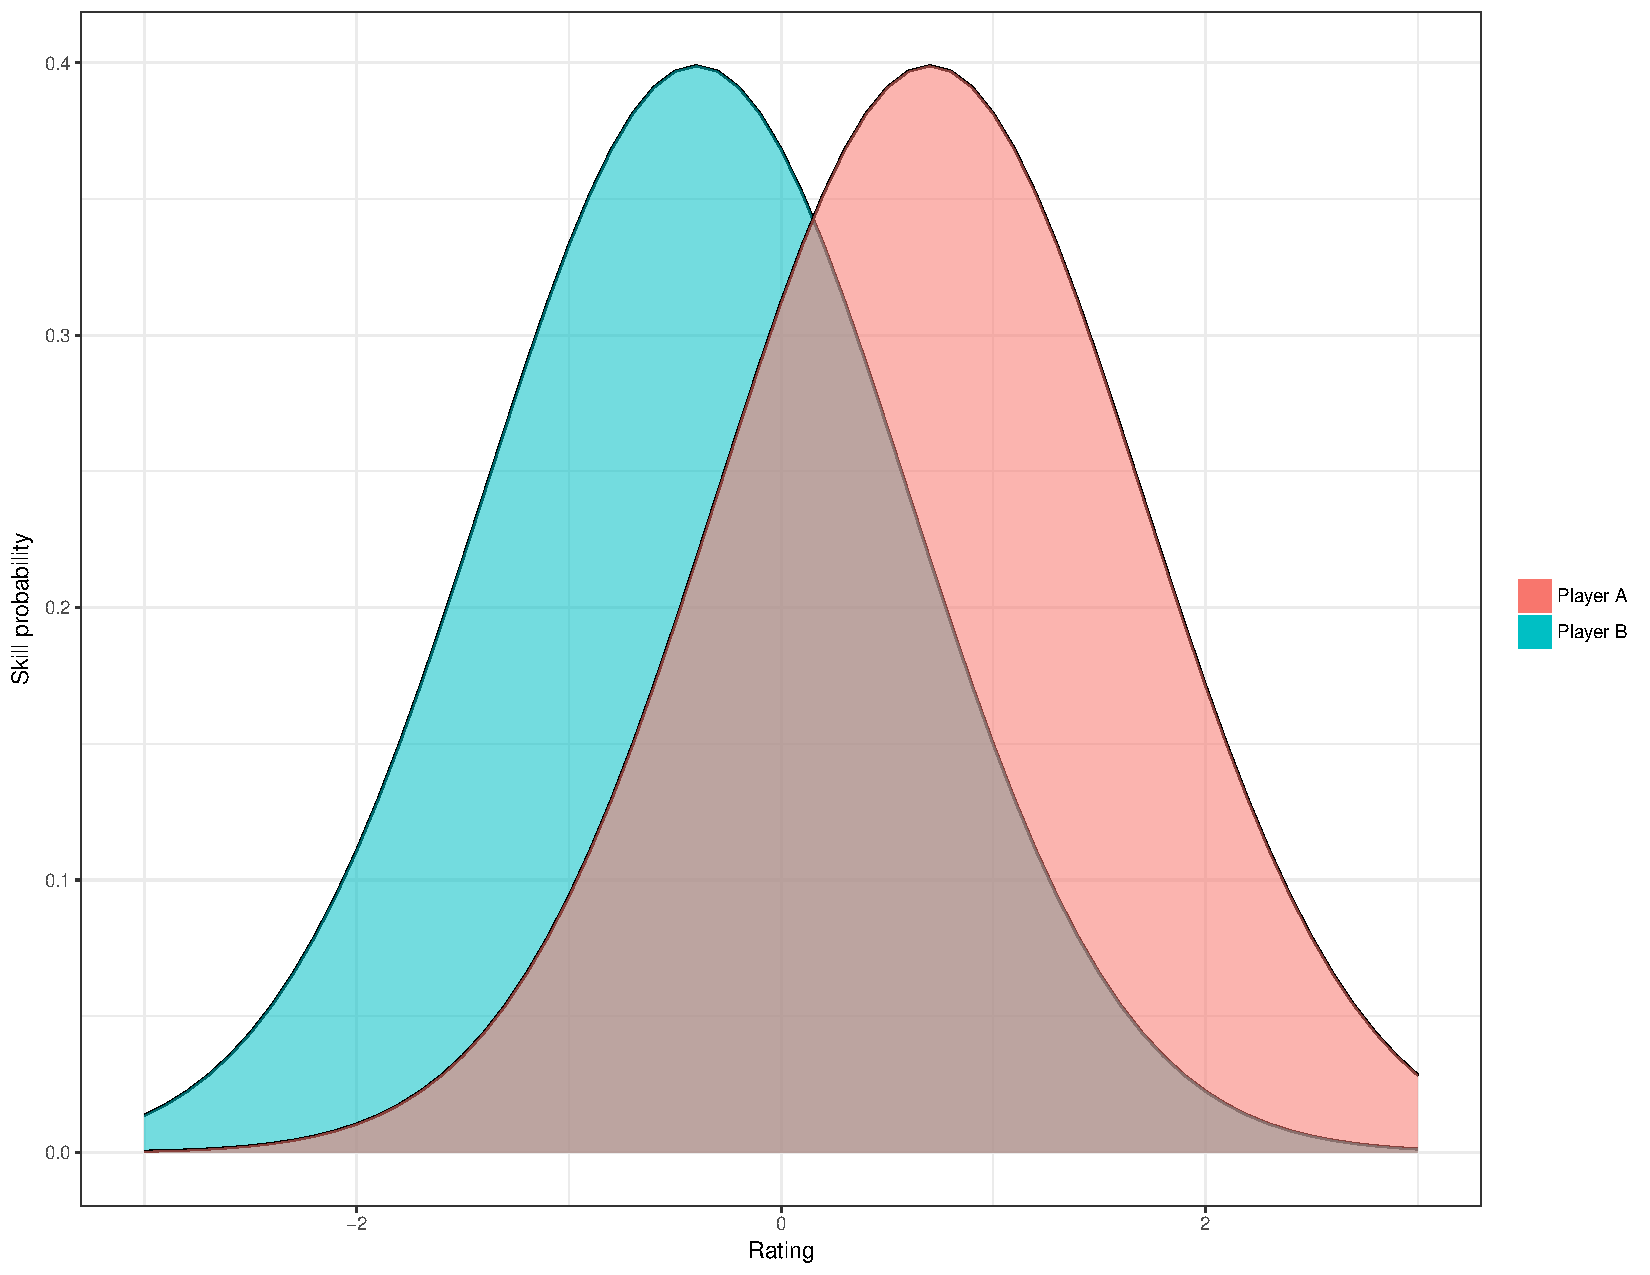
\includegraphics[width=.8\linewidth]{figs/players_skill_distribution}
\caption{Standard normal distribution of skills of players A and B}
\end{figure}

\noindent Hence the distribution of the outcome obtained by substracting distributions:
\begin{figure}[H]
\centering
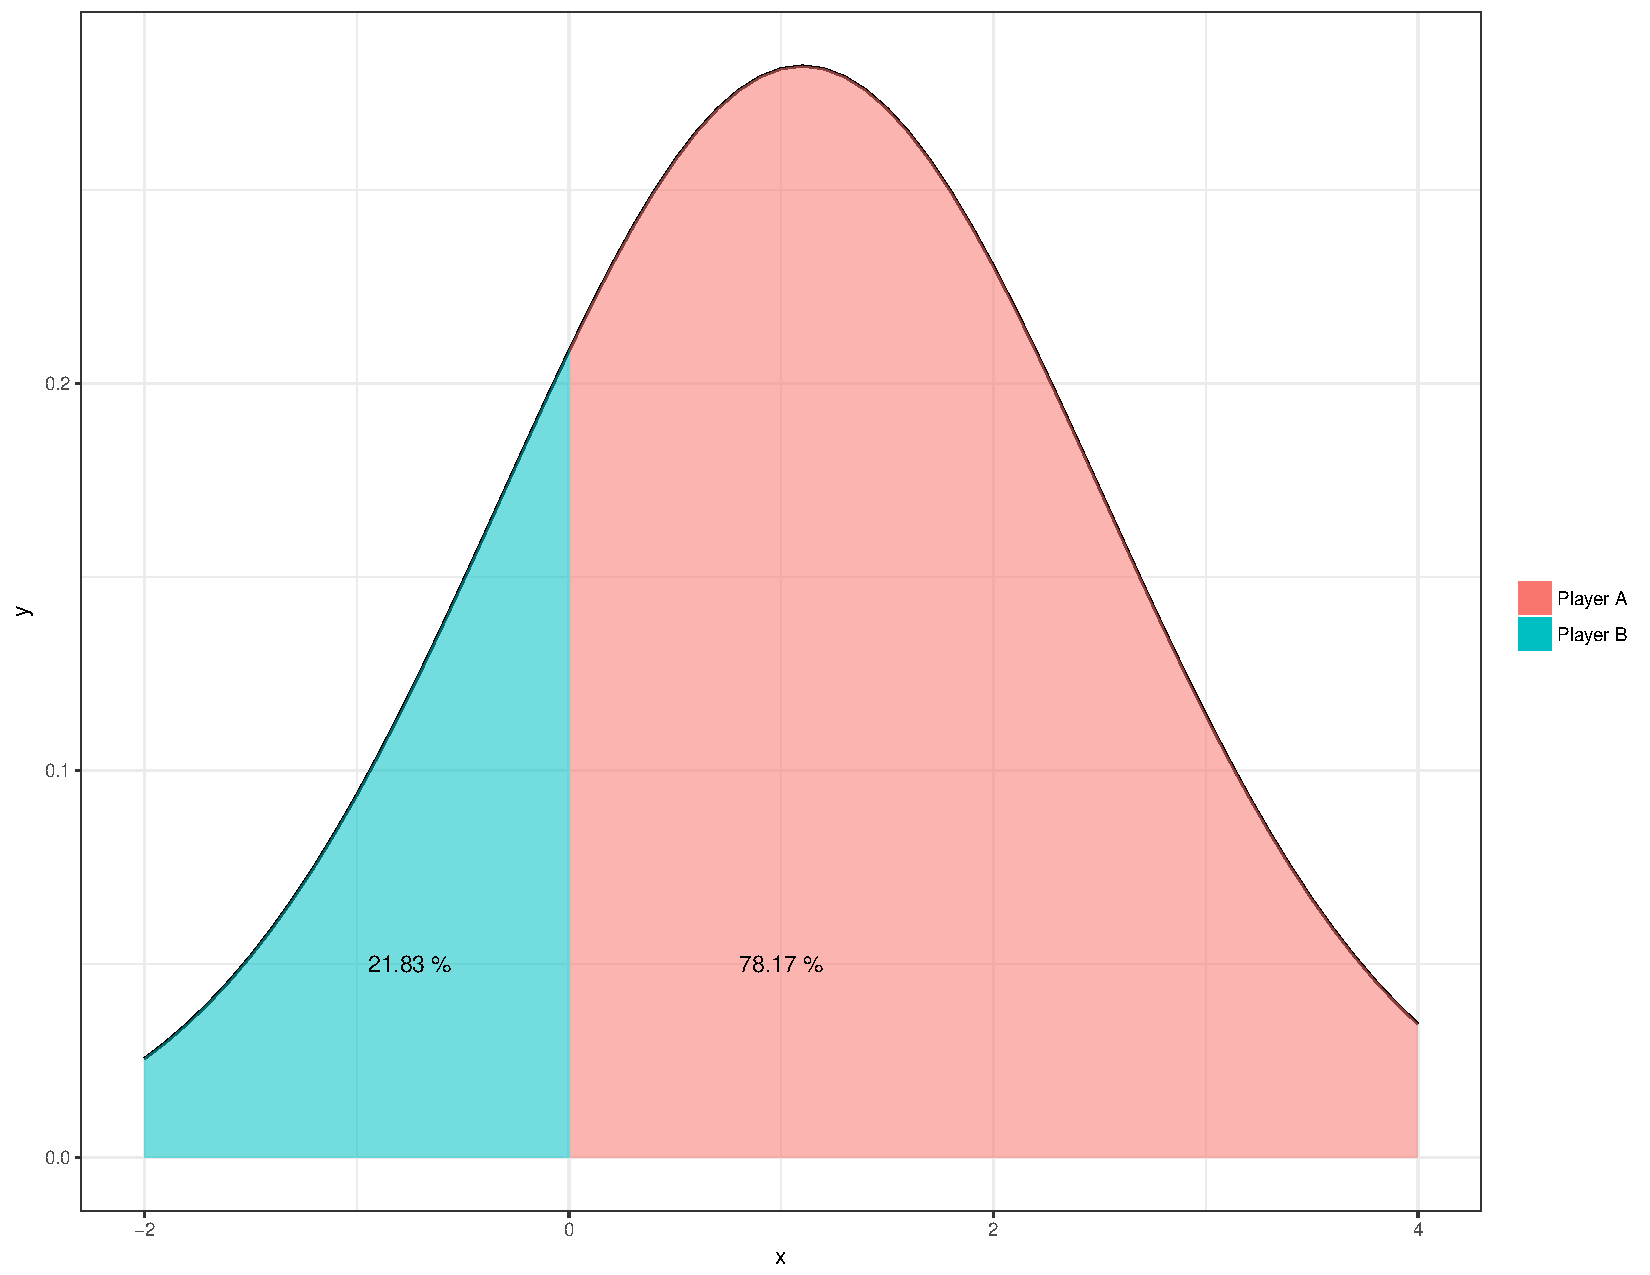
\includegraphics[width=.8\linewidth]{figs/outcome_distribution}
\caption{Distribution of outcome of a match}
\end{figure}

Therefore, the probability of player A defeating player B based on the certainty of their skills being -0.4 and 0.7, respectively, is 78.17\%.
\end{example}

\section{Outline of the thesis}
To complete the introductory chapter, we provide an overview of the chapters presented in the thesis. 

In \autoref{ch:online_ranking}, we will thoroughly describe the Elo algorithm followed by an extension for team ranking. Moreover, we will introduce several methods for improving the prediction ability of the Elo algorithm as well as techniques for adjusting the algorithm to used data.

In \autoref{ch:batch_ranking}, we will describe three algorithms that approach the problem of predicting outcomes of matches by processing previous matches. While the sections of Graph-based algorithms and Supervised Learning approach introduce state-of-the-art approaches for the task, the Maximum-likelihood method is our proposal for dealing with the problem statistics-wise.

In \autoref{ch:realisation}, we provide a description of the API of several ranking algorithms built for an easier access to the methods introduced throughout the thesis. The API is used in the demo web application to demonstrate its functionality. Moreover, a brief description of the scripts used to generate results as seen in the thesis is provided.

Finally, in \autoref{ch:conclusion}, we provide an overview of introduced algorithms followed by a conclusion derived from the work. Further, a table of results describing key features of said algorithms is presented alongside with their ability to predict outcomes of matches.